\title{Warm-Up for April 20th, 2022}
\author{Dr. Jordan Hanson - Whittier College Dept. of Physics and Astronomy}
\date{\today}
\documentclass[12pt]{article}
\usepackage[a4paper, total={18cm, 27cm}]{geometry}
\usepackage{graphicx}
\usepackage{amsmath}
\usepackage{subcaption}
\usepackage{bm}
\def\rcurs{{\mbox{$\resizebox{.16in}{.08in}{
\includegraphics{ScriptR}}$}}}
\def\brcurs{{\mbox{$\resizebox{.16in}{.08in}{
\includegraphics{BoldR}}$}}}
\def\hrcurs{{\mbox{$\hat \brcurs$}}}
 
\begin{document}
\maketitle
\small
\section{Memory Bank}
\begin{enumerate}
\item Definitions of bound currents, given the \textit{magnetization} $\mathbf{M}$ (magnetic dipole moment per unit volume).
\begin{align}
\mathbf{J}_b &= \nabla \times \mathbf{M} \\
\mathbf{K}_b &= \mathbf{M} \times \hat{\mathbf{n}}
\end{align}
\end{enumerate}

\section{Bound Currents and Magnetization}

\begin{enumerate}
\item An infinitely long circular cylinder (Fig. \ref{fig:1}) carries a uniform magnetization $\mathbf{M}$ parallel to its axis.  Find the magnetic field (due to $\mathbf{M}$) inside and outside the cylinder.  \textit{[Hint: let $\mathbf{M} = M\hat{\mathbf{z}}$, and try to vizualize the current.]}
\end{enumerate}

\begin{figure}
\centering
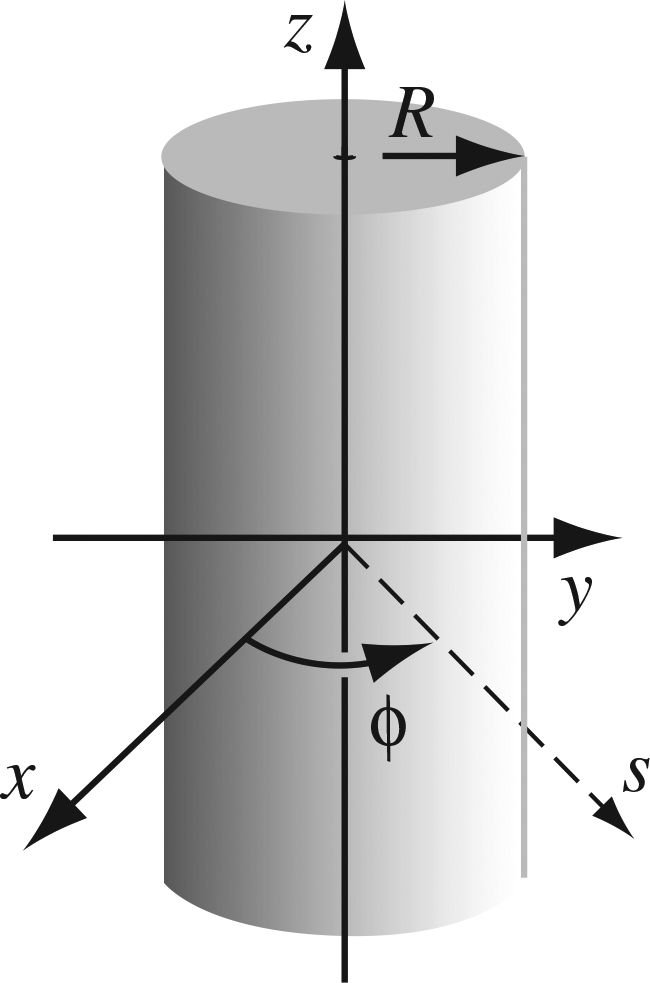
\includegraphics[width=0.2\textwidth]{figures/6_13.jpg}
\caption{\label{fig:1} A circular cylinder with uniform magnetization along the z-axis.}
\end{figure}

\end{document}